
\SGARefTarget{sga3:x:chapter:x}\chapter*{Exposé X\\
Characterization and Classification\\
of Groups of Multiplicative Type}
\addcontentsline{toc}{chapter}{Exposé X. Characterization and
Classification of Groups of Multiplicative Type}
\markboth{EXPOSÉ X. GROUPS OF MULTIPLICATIVE TYPE}
  {EXPOSÉ X. GROUPS OF MULTIPLICATIVE TYPE}

\begin{center}
  \textit{by A. Grothendieck}
\end{center}

\SGARefTarget{sga3:x:section:1}\section*{1. Classification of Isotrivial
Groups. Case of a Base Field}
\addcontentsline{toc}{section}{1. Classification of Isotrivial Groups.
Case of a Base Field}

Recall (\SGARefLink{sga3:ix:definition:1:1}{IX~1.1}) that a group of multiplicative type \(H\) over the
prescheme \(S\) is said to be \emph{isotrivial} if there exists a finite
étale surjective morphism \(S'\to S\) such that
\(H'=H\times_S S'\) is diagonalizable. When \(S\) is connected,
\(S'\) decomposes as a finite disjoint sum of connected components
\(S'_i\), and hence, after replacing \(S'\) by one of the \(S'_i\), we
may suppose that \(S'\) is connected. Finally, \(S'\) can be dominated
by a connected finite étale \(S'_1\) that is Galois, that is, a
principal homogeneous bundle over \(S\) with group \(\Gamma_S\), where
\(\Gamma\) is an ordinary finite group (cf.\ SGA~1, V, nos.~7 and~3
when \(S\) is locally noetherian, and EGA~IV\textsubscript{4}, 18.2.9
in general).
We suppose \(S'\) chosen in this way and propose to determine the
groups of multiplicative type \(H\) over \(S\) that are
``trivialized'' by \(S'\), that is, those for which
\(H'=H\times_S S'\) is diagonalizable.
By descent theory (cf.\ SGA~1, VIII, \SGARefLink{sga3:viii:corollary:5:4}{5.4}), the category of such \(H\)
is equivalent to the category of diagonalizable groups \(H'\) over
\(S'\), equipped with actions of \(\Gamma\) on \(H'\) compatible with
the actions of \(\Gamma\) on \(S'\). (N.B. Since the groups under
consideration are affine over the base, every descent datum here is
effective; cf.\ SGA~1, VIII, \SGARefLink{sga3:viii:proposition:2:1}{2.1}.) Since \(S'\) is connected, the
contravariant functor
\[
  M\longmapsto D_{S'}(M)
\]
is an anti-equivalence from the category of ordinary commutative
groups to the category of diagonalizable groups over \(S'\)
(cf.\ \SGARefLink{sga3:viii:corollary:1:6}{VIII~1.6}); a quasi-inverse is
\[
  H\longmapsto
  \operatorname{Hom}_{S'\text{-}\mathrm{gr}}(H,\mathbb G_{m,S'}).
\]

\medskip
\noindent\SGARefTarget{sga3:x:proposition:1:1}%
\textbf{Proposition 1.1.} ---
\textit{Let \(S\) be a connected prescheme and let \(S'\) be a
connected principal cover of \(S\) with finite group \(\Gamma\). Then
the category of groups of multiplicative type over \(S\) split by
\(S'\) is
anti-equivalent to the category of \(\Gamma\)-modules, that is, of
ordinary commutative groups \(M\) equipped with a homomorphism
\[
  \Gamma\longrightarrow\operatorname{Aut}_{\mathrm{gr}}(M).
\]}

The following standard consequence results.

\medskip
\noindent\SGARefTarget{sga3:x:corollary:1:2}%
\textbf{Corollary 1.2.} ---
\textit{Let \(S\) be a connected prescheme, and let
\(\xi:\operatorname{Spec}(\Omega)\to S\) be a ``geometric point'' of
\(S\), that is, a morphism into \(S\) from the spectrum of an
algebraically closed field \(\Omega\). Consider the fundamental group
of \(S\) at \(\xi\) (cf.\ SGA~1, V, no.~7):
\[
  \pi=\pi_1(S,\xi).
\]
Then the category of isotrivial groups of multiplicative type \(H\)
over \(S\) is anti-equivalent to the category of ``Galois modules''
under \(\pi\), that is, of \(\pi\)-modules \(M\) such that the
stabilizer in \(\pi\) of every element of \(M\) is an open subgroup.}

\textit{Under this correspondence, the group associated with an
isotrivial group of multiplicative type \(H\) is
\[
  M=\operatorname{Hom}_{\Omega\text{-}\mathrm{gr}}
       (H_\xi,\mathbb G_{m,\Omega}),
\]
where \(H_\xi\) is the fiber of \(H\) at \(\xi\); this group is
naturally endowed with an action of \(\pi_1(S,\xi)\).}

\medskip
\noindent\SGARefTarget{sga3:x:remark:1:3}%
\textbf{Remark 1.3.} ---
We shall see below (cf.\ \SGARefLink{sga3:x:theorem:5-16}{5.16}) that if \(S\) is normal, or more
generally geometrically unibranch, then every group of multiplicative
type and of finite type over \(S\) is necessarily isotrivial.
Consequently, the classification principle of \SGARefLink{sga3:x:corollary:1:2}{1.2} applies to groups of
multiplicative type and of finite type over \(S\); they correspond to
Galois \(\pi\)-modules that are of finite type over \(\mathbb Z\). For
the moment, let us confine ourselves to the following result.

\medskip
\noindent\SGARefTarget{sga3:x:proposition:1:4}%
\textbf{Proposition 1.4.} ---
\textit{Let \(k\) be a field and \(H\) a group of multiplicative type
and of finite type over \(k\). Then \(H\) is isotrivial; that is, there
exists a finite separable extension \(k'\) of \(k\) that splits \(H\).}

\textit{Consequently, by \SGARefLink{sga3:x:corollary:1:2}{1.2}, if \(\pi\) is the topological Galois
group of an algebraic closure \(\Omega\) of \(k\), the category of
groups \(H\) of multiplicative type and of finite type over \(k\) is
anti-equivalent to the category of Galois modules \(M\) under \(\pi\)
that are of finite type as \(\mathbb Z\)-modules.}

Since \(H\) is of finite type over \(k\), the ``principle of finite
extension'' (cf.\ EGA~IV\textsubscript{3}, 9.1.4) first gives a finite
extension \(k'\) of \(k\) that splits \(H\). Recall the argument. By
hypothesis, there exist a diagonalizable group \(G\) of finite type
over \(k\), a faithfully flat \(S'\) over
\(S=\operatorname{Spec}(k)\), and an isomorphism of \(S'\)-groups
\[
  H_{S'}\simeq G_{S'}.
\]
After replacing \(S'\) by the residue field of one of its points, we
may suppose that \(S'\) is the spectrum of an extension \(K\) of
\(k\). The field \(K\) is the filtered direct limit of its finitely
generated \(k\)-subalgebras \(A_i\); it follows readily (cf.\
EGA~IV\textsubscript{3}, 8.8.2.4) that the given isomorphism \(u\)
comes, for sufficiently large \(i\), from an \(A_i\)-isomorphism
\[
  u_i:H_{A_i}\simeq G_{A_i}.
\]
By the Nullstellensatz, \(A_i\) has a quotient ring \(k'\) that is a
finite extension of \(k\). Thus \(k'\) splits \(H\).

Now \(k'\) is a radicial extension of a separable extension \(k'_s\)
of \(k\). By \SGARefLink{sga3:ix:corollary:5:4}{IX~5.4}, the isomorphism
\[
  u':H_{k'}\simeq G_{k'}
\]
comes from an isomorphism \(H_{k'_s}\simeq G_{k'_s}\). Thus \(k'_s\)
splits \(H\), proving \SGARefLink{sga3:x:proposition:1:4}{1.4}.

\medskip
\noindent\SGARefTarget{sga3:x:remark:1:5}%
\textbf{Remark 1.5.} ---
Statement \SGARefLink{sga3:x:corollary:1:2}{1.2} gives, in particular, a characterization of the
isotrivial tori over \(S\) of relative dimension \(n\): setting
\(\pi=\pi_1(S,\xi)\), they correspond to classes, up to
``equivalence,'' of representations
\[
  \pi\longrightarrow\operatorname{GL}(n,\mathbb Z)
\]
whose kernel is an open subgroup of \(\pi\).

\medskip
\noindent\SGARefTarget{sga3:x:paragraph:1:6}\textbf{1.6.}
Even when \(S\) is an algebraic curve, there may exist tori over \(S\)
(of relative dimension \(2\)) that are not locally isotrivial (and
\emph{a fortiori} not isotrivial); there may also exist locally
trivial tori that are not isotrivial. (Observe, however, that such
phenomena can occur only when \(S\) is not normal, as already noted in
\SGARefLink{sga3:x:remark:1:3}{1.3}.) For example, let \(S\) be an irreducible algebraic curve (over
an algebraically closed field, to fix ideas) with an ordinary double
point \(a\), let \(S'\) be its normalization, and let \(b\) and \(c\)
be the two points of \(S'\) above \(a\). A connected principal
homogeneous bundle \(P\) over \(S\), with structural group
\(\mathbb Z\), is obtained by attaching infinitely many copies of
\(S'\) according to the diagram
\begin{center}
  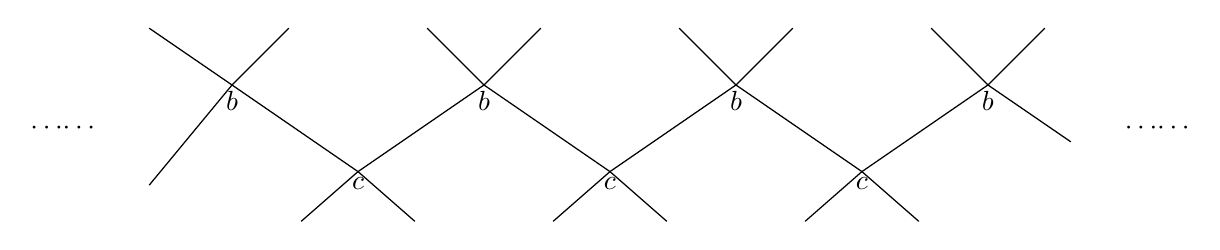
\begin{tikzpicture}[
  x=1cm,
  y=1cm,
  line cap=round,
  line join=round,
  every node/.style={inner sep=1pt}
]
  \coordinate (b1) at (2.8,0.55);
  \coordinate (c1) at (4.4,-0.55);
  \coordinate (b2) at (6.0,0.55);
  \coordinate (c2) at (7.6,-0.55);
  \coordinate (b3) at (9.2,0.55);
  \coordinate (c3) at (10.8,-0.55);
  \coordinate (b4) at (12.4,0.55);

  \draw[line width=.45pt]
    (1.75,1.27) -- (b1) -- (c1) -- (b2) -- (c2) --
    (b3) -- (c3) -- (b4) -- (13.45,-0.17);
  \draw[line width=.45pt] (1.75,-0.72) -- (b1) -- (3.52,1.27);
  \draw[line width=.45pt] (3.68,-1.18) -- (c1) -- (5.12,-1.18);
  \draw[line width=.45pt] (5.28,1.27) -- (b2) -- (6.72,1.27);
  \draw[line width=.45pt] (6.88,-1.18) -- (c2) -- (8.32,-1.18);
  \draw[line width=.45pt] (8.48,1.27) -- (b3) -- (9.92,1.27);
  \draw[line width=.45pt] (10.08,-1.18) -- (c3) -- (11.52,-1.18);
  \draw[line width=.45pt] (11.68,1.27) -- (b4) -- (13.12,1.27);

  \node[below=1pt] at (b1) {$b$};
  \node[below=1pt] at (b2) {$b$};
  \node[below=1pt] at (b3) {$b$};
  \node[below=1pt] at (b4) {$b$};
  \node[below=1pt] at (c1) {$c$};
  \node[below=1pt] at (c2) {$c$};
  \node[below=1pt] at (c3) {$c$};

  \node at (0.65,0) {$\cdots\!\cdots$};
  \node at (14.55,0) {$\cdots\!\cdots$};
\end{tikzpicture}

\end{center}
(N.B. This is a principal bundle for the étale topology.) There is a
homomorphism
\[
  \varphi:\mathbb Z\longrightarrow\operatorname{GL}(2,\mathbb Z),
  \qquad
  \varphi(n)=
  \begin{pmatrix}
    1 & n\\
    0 & 1
  \end{pmatrix},
\]
which makes it possible to construct a torus \(T\) over \(S\), of
relative dimension \(2\), from the trivial torus \(\mathbb G_m^2\)
over \(P\) and the descent datum on it deduced from \(\varphi\).
(N.B. The projection \(P\to S\) is a covering for the étale topology
and \emph{a fortiori} for the canonical topology of
\((\mathbf{Sch})\); the descent datum in question is necessarily
effective because \(\mathbb G_{m,P}^2\) is affine over \(P\).) It is
not difficult to prove that \(T\) is not isotrivial in a neighborhood
of \(a\) (although it is
trivial on \(S-\{a\}\)).

A variant of this construction is obtained by taking for \(S\) a
curve with two irreducible components \(S_1\) and \(S_2\) meeting in
two points \(a'\) and \(a''\). This makes it possible to construct a
connected, locally trivial principal homogeneous bundle \(P\) over
\(S\) with group \(\mathbb Z_S\), and hence an associated torus \(T\)
that is locally trivial but not isotrivial.

\SGARefTarget{sga3:x:section:2}\section*{2. Infinitesimal Variations of
Structure}
\addcontentsline{toc}{section}{2. Infinitesimal Variations of Structure}

\footnote{Editor's note: This ``recall'' has been added for later
references.}
Let us begin by recalling the following result (cf.\ SGA~1, I, 8.3
when \(S\) is locally noetherian, and EGA~IV\textsubscript{4}, 18.1.2
in general).

\medskip
\noindent\SGARefTarget{sga3:x:recall:2:0}\textbf{Recall 2.0.} ---
\textit{Let \(S\) be a prescheme and \(S_0\) a subprescheme with the
same underlying set. Then the functor
\[
  X\longmapsto X_0=X\times_S S_0
\]
is an equivalence between the category of étale preschemes over \(S\)
and the analogous category over \(S_0\).}

\medskip
\noindent\SGARefTarget{sga3:x:proposition:2:1}%
\textbf{Proposition 2.1.} ---
\textit{Let \(S\) be a prescheme and \(S_0\) a subprescheme with the
same underlying set (that is, defined by a nilideal \(\mathscr I\)).
Then the functor
\[
  H\longmapsto H_0=H\times_S S_0
\]
from the category of group preschemes of multiplicative type over
\(S\) to the analogous category over \(S_0\) is fully faithful.}

\textit{Moreover, it induces an equivalence between the category of
quasi-isotrivial groups of multiplicative type over \(S\) and the
analogous category over \(S_0\).}

We first prove full faithfulness, that is, if \(H\) and \(G\) over
\(S\) are of multiplicative type, then
\[
  \operatorname{Hom}_{S\text{-}\mathrm{gr}}(H,G)
  \longrightarrow
  \operatorname{Hom}_{S_0\text{-}\mathrm{gr}}(H_0,G_0)
\]
is bijective. The question is local on \(S\), so we may suppose that
\(S\) is affine. There then exists a faithfully flat quasi-compact
morphism \(S'\to S\) that splits \(H\) and \(G\). Let
\(S''=S'\times_S S'\); write \(H',G'\), respectively \(H'',G''\), for
the groups obtained from \(H,G\) by the base changes \(S'\to S\),
respectively \(S''\to S\). Define \(S'_0\) and \(S''_0\) similarly;
the latter is also isomorphic to \(S'_0\times_{S_0}S'_0\). We obtain a
commutative diagram with exact rows:
\begin{center}
  {\small
\begin{tikzcd}[column sep=2.1em, row sep=3.4em]
  \operatorname{Hom}_{S\text{-}\mathrm{gr.}}(H,G)
    \arrow[r]
    \arrow[d,"u"]
  &
  \operatorname{Hom}_{S'\text{-}\mathrm{gr.}}(H',G')
    \arrow[r,shift left=.65ex]
    \arrow[r,shift right=.65ex]
    \arrow[d,"u'"]
  &
  \operatorname{Hom}_{S''\text{-}\mathrm{gr.}}(H'',G'')
    \arrow[d,"u''"]
  \\
  \operatorname{Hom}_{S_0\text{-}\mathrm{gr.}}(H_0,G_0)
    \arrow[r]
  &
  \operatorname{Hom}_{S'_0\text{-}\mathrm{gr.}}(H'_0,G'_0)
    \arrow[r,shift left=.65ex]
    \arrow[r,shift right=.65ex]
  &
  \operatorname{Hom}_{S''_0\text{-}\mathrm{gr.}}(H''_0,G''_0),
\end{tikzcd}
}

\end{center}
Thus, to prove that \(u\) is bijective, it is enough to prove that
\(u'\) and \(u''\) are bijective. This reduces us to the case where
\(H\) and \(G\) are diagonalizable, hence of the form \(D_S(M)\) and
\(D_S(N)\), where \(M\) and \(N\) are ordinary commutative groups.
Likewise,
\[
  H_0=D_{S_0}(M),\qquad G_0=D_{S_0}(N).
\]
We then have a commutative diagram
\begin{center}
  {\small
\begin{tikzcd}[column sep=3.2em, row sep=3.5em]
  \operatorname{Hom}_{S\text{-}\mathrm{gr.}}(N_S,M_S)
    \arrow[r,"\sim"]
    \arrow[d]
  &
  \operatorname{Hom}_{S\text{-}\mathrm{gr.}}\!\bigl(D_S(M),D_S(N)\bigr)
    \arrow[d]
  \\
  \operatorname{Hom}_{S_0\text{-}\mathrm{gr.}}(N_{S_0},M_{S_0})
    \arrow[r,"\sim"]
  &
  \operatorname{Hom}_{S_0\text{-}\mathrm{gr.}}\!\bigl(D_{S_0}(M),D_{S_0}(N)\bigr),
\end{tikzcd}
}

\end{center}
whose horizontal arrows are isomorphisms by \SGARefLink{sga3:viii:corollary:1:4}{VIII~1.4}. We are therefore
reduced to proving that the homomorphism
\begin{equation}
  \operatorname{Hom}_{S\text{-}\mathrm{gr}}(N_S,M_S)
  \longrightarrow
  \operatorname{Hom}_{S_0\text{-}\mathrm{gr}}(N_{S_0},M_{S_0})
  \tag{x}\label{sga3:x:proposition:2-1:equation:x}
\end{equation}
is bijective; in other words, the functor
\(M_S\mapsto M_{S_0}\), from constant commutative group preschemes
over \(S\) to constant commutative group preschemes over \(S_0\), is
fully faithful. Now \SGARefLink{sga3:x:proposition:2-1:equation:x}{(x)} is also identified with the natural map
\[
  \operatorname{Hom}_{\mathrm{gr}}(N,\Gamma(M_S))
  \longrightarrow
  \operatorname{Hom}_{\mathrm{gr}}(N,\Gamma(M_{S_0}))
\]
deduced from \(\Gamma(M_S)\to\Gamma(M_{S_0})\). The latter map is
plainly bijective, since \(\Gamma(M_S)\), the set of locally constant
maps from \(S\) to \(M\), depends only on the underlying topological
space of \(S\). This proves the desired assertion.

To prove the second assertion of \SGARefLink{sga3:x:proposition:2:1}{2.1}, it remains to show that every
quasi-isotrivial group \(H_0\) of multiplicative type over \(S_0\)
comes from a quasi-isotrivial group \(H\) of multiplicative type over
\(S\). Let \(S'_0\to S_0\) be an étale surjective morphism that splits
\(H_0\).

By \SGARefLink{sga3:x:recall:2:0}{2.0}, there exist an étale morphism \(S'\to S\) and an
\(S_0\)-isomorphism
\[
  S'\times_S S_0\simeq S'_0.
\]
Thus we may suppose that \(S'_0\) is obtained from \(S'\) by
reduction. Since \(H'_0\) is diagonalizable, it is immediately seen
to be isomorphic to the group obtained by the base change
\(S'_0\to S'\) from a diagonalizable group \(H'\) over \(S'\). (N.B.
If \(H'_0=D_{S'_0}(M)\), take \(H'=D_{S'}(M)\).) As usual, set
\[
  S''=S'\times_S S',
  \qquad
  S'''=S'\times_S S'\times_S S',
\]
and similarly define \(S''_0\) and \(S'''_0\) by base change from
\(S\) to \(S_0\). They are also isomorphic to the fibered square and
fibered cube, respectively, of \(S'_0\) over \(S_0\). Applying the
full faithfulness already proved to \((S'',S''_0)\) and
\((S''',S'''_0)\), we see that the natural descent datum on \(H'_0\)
relative to \(S'_0\to S_0\) (cf.\ \SGARefLink{sga3:iv:definition:2:1}{IV~2.1}) comes from a uniquely
determined descent datum on \(H'\) relative to \(S'\to S\). This
descent datum is effective because \(H'\) is affine over \(S'\)
(SGA~1, VIII, \SGARefLink{sga3:viii:proposition:2:1}{2.1}). Hence there exists an \(S\)-group \(H\) such that
\[
  H\times_S S'=H'=D_{S'}(M),
\]
and \(H\) is therefore a quasi-isotrivial group of multiplicative
type.

Using the full-faithfulness result for \((S',S'_0)\), one now checks
readily that the given isomorphism between \(H'_0\) and
\(H'\times_{S'}S'_0\) comes from an isomorphism between \(H_0\) and
\(H\times_S S_0\). (For a more formal presentation of results of this
kind, see Giraud's article in preparation on descent theory.%
\begingroup
\renewcommand{\thefootnote}{\(\ast\)}%
\footnote{Cf.\ J.~Giraud, ``Méthode de la descente,'' \emph{Bull.\
Soc.\ Math.\ France}, Mémoire~2 (1964).}%
\endgroup
\addtocounter{footnote}{-1})

\medskip
\noindent\SGARefTarget{sga3:x:corollary:2:2}%
\textbf{Corollary 2.2.} ---
\textit{Let \(H\) be an \(S\)-group of multiplicative type, and set
\(H_0=H\times_S S_0\). Then \(H\) is quasi-isotrivial (respectively,
locally isotrivial, isotrivial, locally trivial, or trivial) if and
only if \(H_0\) has the corresponding property.}

The ``only if'' direction is immediate. The ``if'' direction has
already been proved in the quasi-isotrivial case: by full
faithfulness, it is enough to know that every quasi-isotrivial group
over \(S_0\) lifts to a quasi-isotrivial group over \(S\). The same
argument applies to ``trivial.'' For ``isotrivial,'' repeat the
argument establishing the second assertion of \SGARefLink{sga3:x:proposition:2:1}{2.1}, but take
\(S'_0\to S_0\) to be finite étale and surjective. The locally
isotrivial and locally trivial cases follow at once from the
isotrivial and trivial cases.

When \(\mathscr I\) is nilpotent, \SGARefLink{sga3:x:corollary:2:2}{2.2} can be generalized slightly
without assuming \emph{a priori} that \(H\) is of multiplicative
type.

\medskip
\noindent\SGARefTarget{sga3:x:corollary:2:3}%
\textbf{Corollary 2.3.} ---
\textit{Suppose that the ideal \(\mathscr I\) defining \(S_0\) is
locally nilpotent. Let \(H\) be a group prescheme over \(S\), flat
over \(S\), and set \(H_0=H\times_S S_0\). Then \(H\) is of
quasi-isotrivial multiplicative type if and only if \(H_0\) is so.}

Suppose that \(H_0\) is of quasi-isotrivial multiplicative type. We
prove that the same is true of \(H\). The question is local for the
étale topology, and by \SGARefLink{sga3:x:recall:2:0}{2.0} the category of étale preschemes over \(S\)
is equivalent to the category of étale preschemes over \(S_0\) by the
functor \(S'\mapsto S'\times_S S_0\). We are therefore immediately
reduced to the case where \(H_0\) is diagonalizable, hence isomorphic
to \(D_{S_0}(M)\). Let \(G=D_S(M)\). We then have an isomorphism
\[
  u_0:H_0\xrightarrow{\sim}G_0.
\]
I claim that \(u_0\) comes from a unique homomorphism \(u:H\to G\),
which is necessarily an isomorphism because \(u_0\) is one, \(H\) and
\(G\) are flat over \(S\), and \(\mathscr I\) is locally
nilpotent.\footnote{Editor's note: Since \(u_0\) is an isomorphism, it
is enough to see that for every \(h\in H\), the morphism
\(\varphi:\mathscr O_{G,u(h)}\to\mathscr O_{H,h}\) is bijective. It is
bijective after reduction modulo
\(\mathscr I=\mathscr I_s\), where \(s\) is the image of \(h\) in
\(S\); hence its cokernel \(C\) satisfies \(C=\mathscr IC\), so
\(C=0\) because \(\mathscr I\) is nilpotent. Since
\(\mathscr O_{H,h}\) is flat
over \(\mathscr O_{S,s}\), the kernel \(K\) of \(\varphi\) likewise
satisfies \(K=\mathscr IK\), and hence \(K=0\).}
This will prove \SGARefLink{sga3:x:corollary:2:3}{2.3}. We have (cf.\ VIII~1~(xxx))
\[
  \operatorname{Hom}_{S\text{-}\mathrm{gr}}(H,G)
  \simeq
  \operatorname{Hom}_{S\text{-}\mathrm{gr}}
  \bigl(M_S,
    \underline{\operatorname{Hom}}_{S\text{-}\mathrm{gr}}
      (H,\mathbb G_{m,S})\bigr),
\]
and the right-hand side is also identified with
\[
  \operatorname{Hom}_{\mathrm{gr}}
  \bigl(M,
    \operatorname{Hom}_{S\text{-}\mathrm{gr}}
      (H,\mathbb G_{m,S})\bigr).
\]
Thus the homomorphism
\begin{equation}
  \operatorname{Hom}_{S\text{-}\mathrm{gr}}(H,G)
  \longrightarrow
  \operatorname{Hom}_{S_0\text{-}\mathrm{gr}}(H_0,G_0)
  \tag{x}\label{sga3:x:corollary:2-3:equation:x}
\end{equation}
is isomorphic to the homomorphism
\[
  \operatorname{Hom}_{\mathrm{gr}}
  \bigl(M,\operatorname{Hom}_{S\text{-}\mathrm{gr}}
    (H,\mathbb G_{m,S})\bigr)
  \longrightarrow
  \operatorname{Hom}_{\mathrm{gr}}
  \bigl(M,\operatorname{Hom}_{S_0\text{-}\mathrm{gr}}
    (H_0,\mathbb G_{m,S_0})\bigr)
\]
deduced from the restriction homomorphism
\begin{equation}
  \operatorname{Hom}_{S\text{-}\mathrm{gr}}(H,\mathbb G_{m,S})
  \longrightarrow
  \operatorname{Hom}_{S_0\text{-}\mathrm{gr}}
    (H_0,\mathbb G_{m,S_0}).
  \tag{xx}\label{sga3:x:corollary:2-3:equation:xx}
\end{equation}
It is therefore enough to prove that \SGARefLink{sga3:x:corollary:2-3:equation:xx}{(xx)} is bijective. The question
is local on \(S\), so we may suppose that \(S\) is affine. Since
\(\mathbb G_{m,S}\) is commutative and smooth over \(S\), \SGARefLink{sga3:ix:theorem:3:6}{IX~3.6}
applies and completes the proof.

\medskip
\noindent\SGARefTarget{sga3:x:corollary:2:4}%
\textbf{Corollary 2.4.} ---
\textit{Let \(A\) be an artinian local ring with residue field \(k\),
\(S=\operatorname{Spec}(A)\), and \(S_0=\operatorname{Spec}(k)\).}
\begin{enumerate}
\item[\SGAInlineRefTarget{sga3:x:corollary:2:4:item:i}(i)]\textit{\footnote{Editor's note: The statement has been
rewritten, retaining only the nontrivial implication in order to
highlight it.} Let \(H\) be an \(S\)-group prescheme, flat and locally
of finite type, such that \(H_0=H\times_S S_0\) is of multiplicative
type. Then \(H\) is of multiplicative type, of finite type, and
isotrivial. In particular, every \(S\)-group prescheme \(H\) of
multiplicative type and of finite type is isotrivial.}
\item[\SGAInlineRefTarget{sga3:x:corollary:2:4:item:ii}(ii)]\textit{The functor \(H\mapsto H_0\) is an equivalence
between the category of groups of multiplicative type and of finite
type over \(A\) and the analogous category over \(k\).}
\end{enumerate}

Indeed, let \(H\) be as in \SGARefLink{sga3:x:corollary:2:4:item:i}{(i)}. Then \(H_0\) is of multiplicative type
and locally of finite type, hence of finite type, and therefore
isotrivial by \SGARefLink{sga3:x:proposition:1:4}{1.4}. By \SGARefLink{sga3:x:corollary:2:3}{2.3} and \SGARefLink{sga3:x:corollary:2:2}{2.2}, \(H\) is consequently of
multiplicative type (and hence of finite type) and isotrivial.
Assertion \SGARefLink{sga3:x:corollary:2:4:item:ii}{(ii)} now follows from \SGARefLink{sga3:x:proposition:2:1}{2.1}.

\medskip
\noindent\SGARefTarget{sga3:x:corollary:2:5}%
\textbf{Corollary 2.5.} ---
\textit{Let \(S'\to S\) be a faithfully flat radicial morphism.}
\begin{enumerate}
\item[(i)]\textit{The functor
\[
  H\longmapsto H'=H\times_S S'
\]
from the category of groups of multiplicative type over \(S\) to the
analogous category over \(S'\) is fully faithful. Moreover, it induces
an equivalence between the subcategories of quasi-isotrivial groups
of multiplicative type.}
\item[(ii)]\textit{If \(H\) is of multiplicative type, then \(H\) is
quasi-isotrivial (respectively, locally isotrivial, isotrivial,
locally trivial, or trivial) if and only if \(H'\) has the
corresponding property.}
\end{enumerate}

Indeed, let
\[
  S''=S'\times_S S',
  \qquad
  S'''=S'\times_S S'\times_S S'.
\]
The assumption that \(S'\to S\) is radicial implies that the diagonal
immersions \(S'\to S''\) and \(S'\to S'''\) are surjective, so base
change by either immersion is governed by \SGARefLink{sga3:x:proposition:2:1}{2.1} and \SGARefLink{sga3:x:corollary:2:2}{2.2}. Taking into
account that \(S'\to S\) is a morphism of effective descent for the
fibered category of groups of multiplicative type over preschemes
(because it is faithfully flat and quasi-compact), the assertion follows formally
from \SGARefLink{sga3:x:proposition:2:1}{2.1} and \SGARefLink{sga3:x:corollary:2:2}{2.2} (cf.\ the already cited article of Giraud for a
formal argument).

\SGARefTarget{sga3:x:section:3}\section*{3. Finite Variations of
Structure: Complete Base Ring}
\addcontentsline{toc}{section}{3. Finite Variations of Structure:
Complete Base Ring}

\medskip
\noindent\SGARefTarget{sga3:x:lemma:3:1}\textbf{Lemma 3.1.} ---
\textit{Let \(A\) be a noetherian ring equipped with an ideal \(I\)
such that \(A\) is separated and complete for the \(I\)-adic topology;
set \(S=\operatorname{Spec}(A)\) and
\(S_0=\operatorname{Spec}(A/I)\). Let \(G\) and \(H\) be two
\(S\)-group preschemes, with \(G\) of multiplicative type and
isotrivial, and with \(H\) affine over \(S\), flat over \(S\) at the
points of \(H_0=H\times_S S_0\), where \(H_0\) is of
quasi-isotrivial multiplicative type. Then the natural map
\[
  \operatorname{Hom}_{S\text{-}\mathrm{gr}}(G,H)
  \longrightarrow
  \operatorname{Hom}_{S_0\text{-}\mathrm{gr}}(G_0,H_0)
\]
is bijective.}

For every integer \(n\geq 0\), let
\[
  S_n=\operatorname{Spec}(A/I^{n+1}),
\]
and let \(G_n,H_n\) be obtained from \(G,H\) by the base change
\(S_n\to S\). Since \(G/S\) is of isotrivial multiplicative type and
\(H\) is affine over \(S\), \SGARefLink{sga3:ix:theorem:7:1}{IX~7.1} shows that the natural
homomorphism
\[
  \operatorname{Hom}_{S\text{-}\mathrm{gr}}(G,H)
  \longrightarrow
  \varprojlim_n
  \operatorname{Hom}_{S_n\text{-}\mathrm{gr}}(G_n,H_n)
\]
is bijective. On the other hand, \SGARefLink{sga3:x:corollary:2:3}{2.3} shows that the \(H_n\) are of
quasi-isotrivial multiplicative type, and \SGARefLink{sga3:x:proposition:2:1}{2.1} shows that all
transition homomorphisms in the inverse system
\[
  \bigl(
    \operatorname{Hom}_{S_n\text{-}\mathrm{gr}}(G_n,H_n)
  \bigr)_n
\]
are isomorphisms. \SGARefLink{sga3:x:lemma:3:1}{Lemma~3.1} follows at once.

\medskip
\noindent\SGARefTarget{sga3:x:theorem:3:2}%
\textbf{Theorem 3.2.} ---
\textit{Let \(A\) be a noetherian ring equipped with an ideal \(I\)
such that \(A\) is separated and complete for the \(I\)-adic topology,
and set \(S=\operatorname{Spec}(A)\) and
\(S_0=\operatorname{Spec}(A/I)\). Then:}
\begin{enumerate}
\item[\SGAInlineRefTarget{sga3:x:theorem:3:2:item:i}(i)]\textit{The functor
\[
  H\longmapsto H_0=H\times_S S_0
\]
is an equivalence between the category of isotrivial groups of
multiplicative type over \(S\) and the analogous category over
\(S_0\).}
\item[\SGAInlineRefTarget{sga3:x:theorem:3:2:item:ii}(ii)]\textit{Let \(H\) be an \(S\)-group of multiplicative type
and of finite type. Then \(H\) is isotrivial if and only if \(H_0\)
is isotrivial.}
\end{enumerate}

\textit{Proof.}
For \SGARefLink{sga3:x:theorem:3:2:item:i}{(i)}, one may either repeat the proof of \SGARefLink{sga3:x:proposition:2:1}{2.1} or use \SGARefLink{sga3:x:corollary:1:2}{1.2}. In either
case one uses the fact that the functor
\[
  S'\longmapsto S'_0=S'\times_S S_0
\]
from the category of finite étale schemes over \(S\) to the category
of finite étale schemes over \(S_0\) is an equivalence (SGA~1, I,
\SGARefLink{sga3:x:lemma:8-4}{8.4}). Equivalently, after reducing to the case where \(S\) is
connected (that is, \(S_0\) is connected) and choosing a geometric
point \(\xi\) of \(S_0\), the canonical homomorphism
\[
  \pi_1(S_0,\xi)\longrightarrow\pi_1(S,\xi)
\]
is an isomorphism.

We prove \SGARefLink{sga3:x:theorem:3:2:item:ii}{(ii)}, namely that if \(H_0\) is isotrivial, then \(H\) is
isotrivial. By \SGARefLink{sga3:x:theorem:3:2:item:i}{(i)}, there exist an isotrivial group \(G\) of
multiplicative type over \(S\) and an \(S_0\)-isomorphism
\[
  u_0:G_0\xrightarrow{\sim}H_0.
\]
\footnote{\label{fnref:X-12}Editor's note: The original has been expanded in what
follows.}
Since \(H\) is of finite type, so are \(H_0\) and \(G_0\). Therefore,
by \SGARefLink{sga3:ix:proposition:2:1}{IX~2.1}~b), the type of \(G\) at every point of \(S\) is a
finitely generated abelian group, and hence \(G\) is of finite type
over \(S\). Moreover, by \SGARefLink{sga3:x:lemma:3:1}{3.1}, \(u_0\) comes from a homomorphism of
\(S\)-groups
\[
  u:G\longrightarrow H.
\]
Finally, \(G\) and \(H\) are groups of multiplicative type and of
finite type over \(S\), and \(u_0\) is an isomorphism. It follows from
\SGARefLink{sga3:ix:corollary:2:9}{IX~2.9} that \(u\) is an isomorphism, since every neighborhood of
\(S_0\) in \(S\) is equal to \(S\).

\medskip
\noindent\SGARefTarget{sga3:x:corollary:3:3}%
\textbf{Corollary 3.3.} ---
\textit{Let \(A\) be a complete noetherian local ring with residue
field \(k\).}
\begin{enumerate}
\item[\SGAInlineRefTarget{sga3:x:corollary:3:3:item:i}(i)]\textit{Every group of multiplicative type and of finite
type over \(A\) is isotrivial.}
\item[(ii)]\textit{The functor
\[
  H\longmapsto H\otimes_A k=H_0
\]
is an equivalence between the categories of groups of multiplicative
type and of finite type over \(A\) and over \(k\).}
\end{enumerate}

\textsuperscript{\normalfont\ref{fnref:X-12}}
First, \SGARefLink{sga3:x:corollary:3:3:item:i}{(i)} follows from \SGARefLink{sga3:x:theorem:3:2}{3.2}~\SGARefLink{sga3:x:theorem:3:2:item:ii}{(ii)} and \SGARefLink{sga3:x:proposition:1:4}{1.4}. Then \SGARefLink{sga3:x:theorem:3:2:item:ii}{(ii)} follows from
\SGARefLink{sga3:x:theorem:3:2}{3.2}~\SGARefLink{sga3:x:theorem:3:2:item:i}{(i)}, taking into account that \(H\) is of finite type if and only
if \(H_0\) is of finite type (cf.\ the proof of \SGARefLink{sga3:x:theorem:3:2}{3.2}~\SGARefLink{sga3:x:theorem:3:2:item:ii}{(ii)}).

\medskip
\noindent\SGARefTarget{sga3:x:remark:3:3:1}%
\textbf{Remark 3.3.1.} ---
By \SGARefLink{sga3:x:proposition:1:4}{1.4}, statement \SGARefLink{sga3:x:corollary:3:3}{3.3} gives a complete classification of groups of
multiplicative type and of finite type over \(A\) in terms of the
topological Galois group of an algebraic closure \(\Omega\) of \(k\).

\medskip
\noindent\SGARefTarget{sga3:x:remarks:3:4}%
\textbf{Remarks 3.4.} ---
Under the hypotheses of \SGARefLink{sga3:x:theorem:3:2}{3.2} (that is, \(A\) noetherian, separated and
complete for the \(I\)-adic topology, with no further hypothesis on
\(A/I\)), it will follow from no.~5 that the functor
\[
  H\longmapsto H_0
\]
from the category of groups of multiplicative type and of finite type
over \(S\) to the analogous category over \(S_0\) is still fully
faithful, without any isotriviality hypothesis.

It is not, however, essentially surjective in general. Indeed, there
may exist a group \(H_0\) of multiplicative type and of finite type
over \(S_0\), even locally trivial if desired (but not isotrivial),
that does not arise by reduction from a group \(H\) of multiplicative
type over \(S\).

To see this, take either example from \SGARefLink{sga3:x:paragraph:1:6}{1.6} of a non-isotrivial group of
multiplicative type over a nonnormal curve. The curve may plainly be
taken affine, say \(S_0\), and embedded in affine \(2\)-space; it is
therefore defined by an ideal \(J\) in \(k[X,Y]\). Take \(A\) to be
the completion of \(k[X,Y]\) for the \(J\)-adic topology. Then \(A\)
is a regular ring of dimension \(2\), and \emph{a fortiori} normal.
We shall see in \SGARefLink{sga3:x:theorem:5-16}{5.16} that every group of multiplicative type and of
finite type over \(S=\operatorname{Spec}(A)\) is consequently
isotrivial. Thus \(H_0\), being of finite type and non-isotrivial,
cannot come from a group \(H\) of multiplicative type over \(S\),
since such an \(H\) would necessarily be of finite type and hence
isotrivial.

\medskip
\noindent\SGARefTarget{sga3:x:lemma:3:5}\textbf{Lemma 3.5.}%
\begingroup
\renewcommand{\thefootnote}{\(\ast\)}%
\footnote{Cf.\ also \(\mathrm{VI}_{\mathrm B}\), \SGARefLink{sga3:x:corollary:2:5}{2.5}, for more
systematic developments of this kind.}%
\endgroup
\addtocounter{footnote}{-1}
---
\textit{Let \(S\) be a prescheme and
\(u:G\to H\) a homomorphism of \(S\)-group preschemes that are
locally of finite presentation and flat over \(S\). Let \(U\) be the
set of \(s\in S\) such that the homomorphism induced on the fibers,
\[
  u_s:G_s\longrightarrow H_s,
\]
is flat (respectively, smooth, unramified, étale, or quasi-finite).
Then \(U\) is open, and the restriction
\[
  u|_U:G|_U\longrightarrow H|_U
\]
is flat (respectively, smooth, unramified, étale, or quasi-finite).}

Let \(V\) be the set of points at which \(u\) is flat (respectively,
\(\ldots\)). It is known that \(V\) is open (cf.\ SGA~1, I through IV
in the locally noetherian case, and EGA~IV in
general), and
for \(x\in G\) above \(s\in S\), one has \(x\in V\) if and only if
\(u_s:G_s\to H_s\) is flat (respectively, \(\ldots\)) at \(x\)
(same reference; in the flat, smooth, and étale cases, the flatness of
\(G\) and \(H\) over \(S\) is used here). Since \(u_s\) is a
homomorphism of locally algebraic groups, this is also equivalent to
\(u_s\) being flat (respectively, \(\ldots\)) everywhere
(\(\mathrm{VI}_{\mathrm B}\), \SGARefLink{sga3:x:remark:1:3}{1.3}), that is, to \(s\in U\).
Therefore \(U\) is the inverse image of the open set \(V\) under the
unit section of \(G\), and hence is open. Moreover, \(V=G|_U\), so
\(G|_U\to H|_U\) is flat (respectively, \(\ldots\)), completing the
proof. (N.B. In the unramified and quasi-finite cases, the flatness
hypothesis on \(G\) and \(H\) is unnecessary.)

\medskip
\noindent\SGARefTarget{sga3:x:lemma:3:6}\textbf{Lemma 3.6.} ---
\textit{Let \(H\) be a commutative algebraic group over a field \(k\)
that admits an open subgroup \(G\) of multiplicative type. Then the
family of subschemes \({}_nH\), \(n>0\), is schematically dense in
\(H\). In particular, if \({}_nH={}_nG\) for every \(n>0\), then
\(H=G\).}

Here \({}_nH\) denotes the kernel of
\(n\cdot\operatorname{id}_H\).\footnote{Editor's note: The preceding
sentence has been added.}
Let \(\bar{k}\) be an algebraic closure of \(k\). It is enough to show
that the family \(({}_nH_{\bar{k}})_{n>0}\) is schematically dense in
\(H_{\bar{k}}\), for then \(({}_nH)_{n>0}\) is schematically dense in
\(H\) (cf.\ \SGARefLink{sga3:ix:lemma:4:5}{IX~4.5}). We may therefore suppose that \(k\) is
algebraically closed, so that \(G=D_k(M)\), where \(M\) is an ordinary
finitely generated commutative group.

Let
\[
  M_0=M/\operatorname{Torsion}(M).
\]
Then \(T=D_k(M_0)\) is the largest torus contained in \(G\), and
\(H/T\) is finite. Hence \(H(k)/T(k)\) is annihilated by an integer
\(\nu>0\). There exist finitely many \(g_i\in H(k)\) such that
\[
  H=\coprod_i g_i\cdot G,
\]
and \(g_i^\nu\in T(k)\). Since \(k\) is algebraically closed, the map
\(\nu\cdot\operatorname{id}_T\) is surjective on
\[
  T(k)\simeq(k^\times)^d.
\]
After replacing \(g_i\) by \(g_it_i^{-1}\), where \(t_i\in T(k)\)
satisfies \(t_i^\nu=g_i^\nu\), we may therefore suppose that
\(g_i^\nu=1\). If \(n\) is now a multiple of \(\nu\), then
\[
  {}_nH\supset g_i\cdot{}_nG.
\]
As \(n>0\) varies, the family \({}_nG\) is schematically dense in
\(G\) by \SGARefLink{sga3:ix:theorem:4:7}{IX~4.7}, and the conclusion of \SGARefLink{sga3:x:lemma:3:6}{3.6} follows.

\medskip
\noindent\SGARefTarget{sga3:x:theorem:3:7}%
\textbf{Theorem 3.7.} ---
\textit{Let \(A\) be a noetherian ring equipped with an ideal \(I\)
such that \(A\) is separated and complete for the \(I\)-adic topology;
set \(S=\operatorname{Spec}(A)\) and
\(S_0=\operatorname{Spec}(A/I)\). Let \(H\) be an affine
\(S\)-group scheme of finite type, flat over \(S\) at the points of
\(H_0\), such that \(H_0=H\times_S S_0\) is of multiplicative type
and isotrivial. Then there exists an open and closed subgroup \(G\) of
\(H\), of isotrivial multiplicative type (and of finite type), such
that \(G_0=H_0\).}

By \SGARefLink{sga3:x:theorem:3:2}{3.2}~\SGARefLink{sga3:x:theorem:3:2:item:i}{(i)}, there exist an isotrivial group \(G\) of multiplicative
type over \(S\) and an isomorphism
\[
  u_0:G_0\xrightarrow{\sim}H_0.
\]
By \SGARefLink{sga3:x:lemma:3:1}{3.1}, \(u_0\) comes from a unique homomorphism of \(S\)-groups
\[
  u:G\longrightarrow H.
\]
Using \SGARefLink{sga3:ix:corollary:6:6}{IX~6.6}, we see that \(u\) is a monomorphism: if \(U\) is the set
of \(s\in S\) such that \(u_s:G_s\to H_s\) is a monomorphism, then
\(U\) is an open neighborhood of \(S_0\), hence equals \(S\), and
\(G|_U\to H|_U\) is a monomorphism. By \SGARefLink{sga3:ix:corollary:2:5}{IX~2.5}, \(u\) is even a closed
immersion.

Thus \(G\) is of finite type, and therefore of finite presentation,
over \(S\).\footnote{Editor's note: The preceding sentence has been
added.}
Applying \SGARefLink{sga3:x:lemma:3:5}{Lemma~3.5} in the étale case, there is an open neighborhood
\(U\) of \(S_0\), hence \(U=S\), such that \(G|_U\to H|_U\) is étale.
Thus \(u\) is étale and therefore an open immersion, since it is an
étale monomorphism.
This completes the proof.

\medskip
\noindent\SGARefTarget{sga3:x:corollary:3:8}%
\textbf{Corollary 3.8.} ---
\textit{Let \(A\) be a noetherian ring equipped with an ideal \(I\)
such that \(A\) is separated and complete for the \(I\)-adic topology;
set \(S=\operatorname{Spec}(A)\) and
\(S_0=\operatorname{Spec}(A/I)\). Let \(H\) be an \(S\)-group
prescheme of finite type, affine and flat over \(S\).}

\textit{Then \(H\) is of multiplicative type and isotrivial if and
only if \(H_0\) is so and \(H\) satisfies either one of the following
conditions \SGARefLink{sga3:x:corollary:3:8:item:a}{(a)} and \SGARefLink{sga3:x:corollary:3:8:item:b}{(b)}, which are therefore equivalent under the
preceding hypotheses:}
\begin{enumerate}
\item[\SGAInlineRefTarget{sga3:x:corollary:3:8:item:a}(a)]\textit{The fibers of \(H\) are of multiplicative type and
have constant type on each connected component of \(S\).}
\item[\SGAInlineRefTarget{sga3:x:corollary:3:8:item:b}(b)]\textit{\(H\) is commutative and the \({}_nH\), \(n>0\),
are finite over \(S\).}
\end{enumerate}
\textit{Both of these conditions are implied by the following one:}
\begin{enumerate}
\item[\SGAInlineRefTarget{sga3:x:corollary:3:8:item:c}(c)]\textit{The fibers of \(H\) are connected.}
\end{enumerate}

Of course, if \(H\) is of multiplicative type (and isotrivial), then
\SGARefLink{sga3:x:corollary:3:8:item:a}{(a)} and \SGARefLink{sga3:x:corollary:3:8:item:b}{(b)} hold by \SGARefLink{sga3:ix:remark:1:4:1}{IX~1.4.1}~a) and \SGARefLink{sga3:x:proposition:2:1}{2.1}~c). Thus only the ``if''
direction requires proof. We use the subgroup \(G\) provided by \SGARefLink{sga3:x:theorem:3:7}{3.7}.
When \SGARefLink{sga3:x:corollary:3:8:item:c}{(c)} holds, plainly \(G=H\), and there is nothing to prove.

In case \SGARefLink{sga3:x:corollary:3:8:item:b}{(b)}, the immersion \(u:G\to H\) induces an open immersion
\[
  {}_nu:{}_nG\longrightarrow{}_nH
\]
and an isomorphism
\[
  ({}_nG)_0\xrightarrow{\sim}({}_nH)_0.
\]
Since \({}_nH\) is finite over \(S\), it follows at once that
\({}_nu\) is an isomorphism: the complement of its image is finite
over \(S\) and reduces to the empty set. By \SGARefLink{sga3:x:lemma:3:6}{3.6}, the induced
morphisms on fibers
\[
  u_s:G_s\longrightarrow H_s
\]
are isomorphisms. Hence \(u\) is surjective and therefore an
isomorphism.

Finally, in case \SGARefLink{sga3:x:corollary:3:8:item:a}{(a)}, we may suppose that \(S\) is
connected.
It follows that, for every \(s\in S\),
\[
  u_s:G_s\longrightarrow H_s
\]
is a monomorphism of algebraic groups of multiplicative type and of
the same type over \(\kappa(s)\).
Such a homomorphism is necessarily an isomorphism, which again
completes the proof.
After extending the base field, we may suppose that both groups over
\(\kappa(s)\) are diagonalizable. The assertion then follows from
\SGARefLink{sga3:viii:corollary:3:2}{VIII~3.2}~b) and the fact that a surjective homomorphism between
isomorphic finitely generated \(\mathbb Z\)-modules
\[
  M\longrightarrow N
\]
is necessarily bijective.

\medskip
\noindent\SGARefTarget{sga3:x:corollary:3:9}%
\textbf{Corollary 3.9.} ---
\textit{Let \(A\) be a noetherian ring equipped with an ideal \(I\)
such that \(A\) is separated and complete for the \(I\)-adic topology,
set \(S=\operatorname{Spec}(A)\), and let \(H\) be an \(S\)-group
prescheme of finite type, affine and flat over \(S\), with connected
fibers. Then \(H\) is an isotrivial torus if and only if
\(H_0=H\times_S\operatorname{Spec}(A/I)\) is an isotrivial torus.}
